\section{Presential Laboratory}
In this laboratory, for the first time in this semester, we were able to attend to a laboratory in person which allowed us to better understand how to design and implement the band-pass filter that we were proposed to in this laboratory assignment using an OP-AMP and undoubtedly to better understand how this circuit works. So, and in order to compare with the circuits built and the components used on the remote work, we took some photos of the circuit and took notes of some relevant values.\\

First, on when it comes to the circuit, it is very similar to the one used on the remote work analysis, but with some differences due to limitations of the components available on the laboratory. Thus, for this circuit we only used $220nF$ capacitors and to distinguish the part that corresponded to the high-pass filter and to the low-pass filter we used different types of resistors (higher values to the high-pass filter - we used a $1k\Omega$ resistor $R_1$ - and lower values to the low-pass filter - where we used two $1k\Omega$ resistors in parallel to achieve a $500\Omega$ resistor $R_2$). For the resistors $R_3$ and $R_4$ we used $1k\Omega$ and $2k\Omega$, respectively. A scheme of the circuit can be seen in Fig. \ref{fig:esquemalab} and a photo of it in Fig. \ref{fig:fotolab}

\begin{figure}[H]
    \centering
    \includegraphics[width=\linewidth]{presentialscheme.pdf}
    \caption{Scheme of the circuit used on the laboratory.}
    \label{fig:esquemalab}
\end{figure}

\begin{figure}[H]
    \centering
    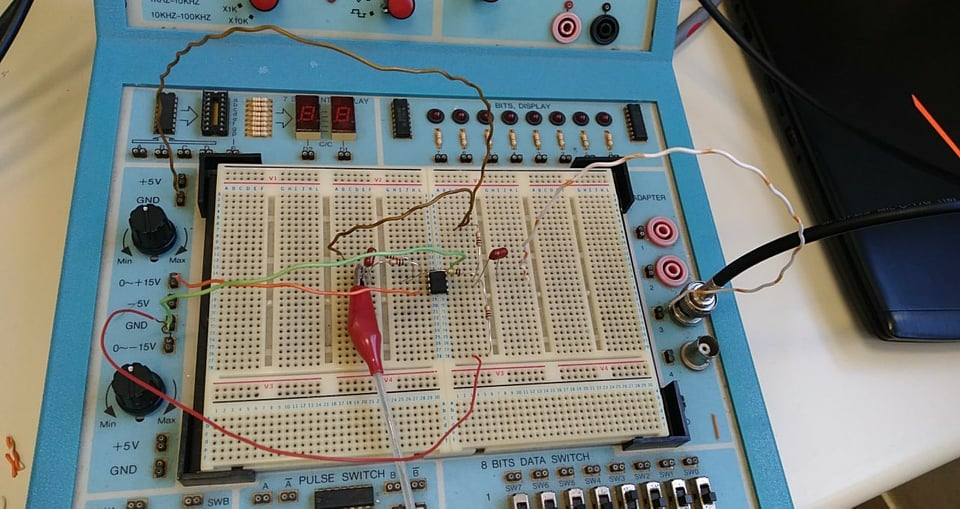
\includegraphics[width=\linewidth]{fotolab.jpg}
    \caption{Photo of the used circuit on the laboratory.}
    \label{fig:fotolab}
\end{figure}

The goals for this work were very similar to the ones for the remote work: amplify an input signal and get a central frequency of $1kHz$ for it. So, in order to better understand how far (or not) we remained from the objectives that were set, we registered the values obtained for the lower and the higher cutoff frequencies (that are, of course, affected with some uncertainty that can't be exactly quantified). The registered values are presented on equation \eqref{values}

\begin{equation}
    f_L = 711Hz \hspace{40px} f_H = 1330Hz
    \label{values}
\end{equation}

Once again, and similarly to what we have done for the remote work, one can find the central frequency of the signal by calculating the geometric mean of the lower and higher cutoff frequencies (definition which results directly from the definition of the transfer function for this circuit). So, we obtain the following value for the central frequency of the signal which is presented on equation \eqref{centraldoff}

\begin{equation}
    central frequency = \sqrt{f_L f_H} \approx 972.435Hz
    \label{centraldoff}
\end{equation}

The value obtained is pretty satisfactory, being sufficiently close enough to the desired value of $1kHz$. To better quantify how far we ended to the desired value, one can calculate the experimental error, which gives an (excellent) value of $\epsilon (\%) = 2.76\%$.